\newenvironment{boxfig}[2]{\begin{figure}[#1]\fbox{\begin{minipage}{0.97\linewidth}
                        \vspace{0.2em}
                        \makebox[0.02\linewidth]{}
                        \begin{minipage}{0.94\linewidth}
            {\small{
                        #2 }}
                        \end{minipage}
                        \vspace{0.2em}
                        \end{minipage}}}{\end{figure}}

\newenvironment{boxfig*}[2]{\begin{figure*}[#1]\fbox{\begin{minipage}{0.97\linewidth}
                        \vspace{0.2em}
                        \makebox[0.02\linewidth]{}
                        \begin{minipage}{0.94\linewidth}
            {\small{
                        #2 }}
                        \end{minipage}
                        \vspace{0.2em}
                        \end{minipage}}}{\end{figure*}}


\newcommand{\alg}[1]{\ensuremath{\mathsf{#1}}}
%\newcommand{\todo}[1]{\textbf{(todo: #1)}}

\newcommand{\binset}{\{0,1\}}
\newcommand{\rfrom}{\ensuremath{\stackrel{\mathrm{R}}{\gets}}}
\newcommand{\from}{\ensuremath{{\gets}}}

\chapter{Secure Function Evaluation with Ordered Binary Decision Diagrams}
\label{chapter:obdd}

\section{Contribution}
\label{sec:obdd-intro}

% Importance of Privacy has spurred interest in privacy-preserving
% protocols.

% Mention importance of BDDs and their applications.
% Describe that it is graph-based data structure.
% Describe our basic contribution.

{\it Ordered Binary Decision Diagrams (OBDDS)}, introduced and
described in section 3.?, are a graph-based representation of Boolean
functions.  We present an
SFE algorithm that directly uses an OBDD representation of the
function $f$ that the two parties want to jointly compute. 

% List of contributions.
Our thesis presents the following contributions:
\begin{itemize}
\item We present a SFE protocol that uses the OBDD representation of
the function to be jointly computed by two parties. Our new protocol along with the
correctness proof is provided in Section~\ref{sec:sfe-obdd}.

\item 
Experimental results based upon a prototype implementation of our
protocol demonstrate that for certain functions, our
implementation results in a smaller encrypted circuit than
the equivalent Yao circuit. For example, for the classic millionaire's problem, our
implementation reduces the bandwidth by approximately $45$\% over the Yao
protocol.  Our
implementation and experimental results are described in
Section~\ref{sec:experiments}.
\end{itemize}

The
advantage of using an OBDD representation over the gate-representation
is that OBDDs are more succinct for certain widely used classes of
functions than the gate representation. For example, among other
functions, our results show the OBDD representation is more efficient
than the gate representation for 8-bit AND, 8-bit addition, and the
millionaire's and billionaire's problems~\cite{Yao:86}.  As a result,
our protocol has reduced bandwidth consumption over the classic Yao
protocol.  Because processor speeds have
increased at a more rapid pace than bandwidth availability over the
past years, network bandwidth is likely to be the bottleneck for a number of applications. In particular, our
protocols are especially useful for applications operating over
networks with limited bandwidth, such as wireless and sensor networks.
Furthermore, we have empirically confirmed this statement by
implementing our protocol and comparing it with the Yao protocol.

In summary, our thesis presents a new SFE protocol that uses the OBDD representation.
The OBDD representation is more efficient for several practical functions of 
interest. For other functions, the circuit description (and therefore
FairPlay) will be more efficient. This protocol presents a generic alternative to 
Boolean circuits that can be used when appropriate. 



\section{Ordered Binary Decision Diagrams (OBDDs)}
\label{sec:OBDDs}

{\it Ordered binary decision diagrams (OBDDs)}  are a canonical 
representation for Boolean formulas~\cite{Bryant:BDD}. They are often
substantially more compact than traditional normal forms, such as
conjunctive normal form (CNF) and disjunctive normal form (DNF), and
they can be manipulated efficiently. Therefore, they are widely used for a
variety of applications in computer-aided design, including symbolic
model checking, verification of combinational logic, and verification of
finite-state concurrent systems~\cite{Clarke:book}.  A detailed
discussion of OBDDs can be found in Bryant's seminal
article~\cite{Bryant:BDD}.


Given a Boolean function $f(x_1,x_2,\cdots,x_n)$ of $n$ variables
$x_1, \cdots, x_n$ and a total ordering on the $n$ variables, the OBDD
for $f$, denoted by $OBDD(f)$, is a rooted, directed acyclic graph
(DAG) with two types of vertices: {\it terminal} and {\it nonterminal}
vertices. $OBDD(f)$ also has the following components:
\begin{itemize}
\item Each vertex
$v$ has a level, denoted by ${\it level}(v)$, between $0$ and $n$. There is a 
distinguished vertex called  {\it root} whose level is $0$. 

\item Each nonterminal vertex $v$ is labeled by a variable ${\it var}(v) \in \{ x_1,\cdots,x_n \}$ and 
has two successors, ${\it low (v)}$ and ${\it high (v)}$. Each
terminal vertex is labeled with either $0$ or $1$. There are only two terminal vertices 
in an OBDD. Moreover, the labeling of vertices respects the total ordering $<$ on the
variables, i.e., if $u$ has a nonterminal successor $v$, then ${\it var}(u) < {\it var}(v)$. 
\end{itemize}
Given an assignment ${\cal A} \; = \; \langle x_1 \leftarrow b_1,
\cdots, x_n \leftarrow b_n \rangle$ to the variables $x_1,\cdots,x_n$
the value of the Boolean function $f(b_1,\cdots,b_n)$ can be found by
starting at the root and following the path where the edges on the
path are labeled with $b_1, \cdots, b_n$. OBDDs can also be used to
represent functions with finite range and domain. Let $g$ be a
function of $n$ Boolean variables with output that can be encoded by
$k$ Boolean variables. The function $g$ can be represented as an array
of $k$ OBDDs where the $i$-th OBDD represents the Boolean function
corresponding to the $i$-th output bit of $g$.  For the rest of the
paper we will assume that the function $f$ is a Boolean function, but
our protocols can be easily extended for the case of functions with a
finite range. We will illustrate OBDDs with an example.
\begin{example}
\label{example:bdd}
\rm
Figure~\ref{fig:OBDD} shows the OBDD for the  function
$f(x_1,x_2,x_3, x_4) \; = \; (x_1 \; = \; x_2) \wedge (x_3 \; = \;
x_4)$ of four variables $x_1,x_2,x_3,x_4$ with the total ordering $x_1
< x_2 < x_3 < x_4$.\footnote{OBDDs are sensitive to variable
ordering, e.g., with the ordering $x_1 < x_3 < x_2 < x_4$ the OBDD for
$(x_1 \; = \; x_2) \wedge (x_3 \; = \; x_4)$ has $11$ nodes.}  Notice that the ordering of
the labels on the vertices on any path from the root to the terminals
of the OBDD corresponds to the total ordering of the Boolean
variables. Consider the assignment $\langle x_1 \leftarrow 1, x_2
\leftarrow 1, x_3 \leftarrow 0, x_4 \leftarrow 0 \rangle$.  In the
OBDD shown in Figure~\ref{fig:OBDD}, if we start at the root and
follow the edges corresponding to the assignment, we end up at the
terminal vertex labeled with $1$. Therefore, the value of $f(1,1,0,0)$
is $1$.
\end{example}

\begin{figure}
\begin{minipage}{3in}
\centering
\fbox{\epsfysize=3.2in \epsfbox{obdd/figures/bdd-fig1.pdf}}
\caption{OBDD for the function $f(x_1,x_2,x_3, x_4) \; = \; (x_1 \; = \; x_2) \wedge (x_3 \; = \;
x_4)$.}
\label{fig:OBDD}
\end{minipage}
\hfill
\begin{minipage}{3in}
\centering
\fbox{\epsfysize=2.5in \epsfbox{obdd/figures/bdd-fig2.pdf}}
\caption{OBDD for the restriction $f \mid_{x_1 \leftarrow 1, x_3 \leftarrow 0}$ where
 $f(x_1,x_2,x_3, x_4) \; = \; (x_1 \; = \; x_2) \wedge (x_3 \; = \;
x_4)$.}
\label{fig:OBDD-reduced}
\end{minipage}
\end{figure}


One of the advantages of OBDDs is that they can be manipulated
efficiently, i.e., given OBDDs for $f$ and $g$, OBDDs for $f \wedge
g$, $f \vee g$, and $\neg f$ can be computed efficiently. We now
describe an operation called {\it restriction}, which is used in our
protocol.  Given a $n$ variable Boolean function
$f(x_1,x_2,\cdots,x_n)$ and a Boolean value $b$, $f
\mid_{x_i \leftarrow b}$ is a Boolean function of $n-1$ variables
$x_1, \cdots, x_{i-1},x_{i+1},\cdots,x_n$ defined as follows:\\
$f \mid_{x_i \leftarrow b} (x_1, \cdots, x_{i-1},x_{i+1},\cdots,x_n)$ is
equal to \\ $f(x_1, \cdots, x_{i-1},b,x_{i+1},\cdots,x_n)$.
Essentially $f \mid_{x_i \leftarrow b}$ is the function obtained by substituting
the value $b$ for the variable $x_i$ in the function $f$. 
Given the OBDD for $f$, the $OBDD$ for $f \mid_{x_i \leftarrow b}$ can
be efficiently computed~\cite[Section 4]{Bryant:BDD}.  The restriction
operation can be extended to multiple variables in a
straightforward manner, e.g., $f \mid_{x_i \leftarrow b, x_j \leftarrow b'}$
can be computed as $(f \mid_{x_i \leftarrow b}) \mid_{x_j \leftarrow b'}$. We
explain the algorithm using our example; the reader is referred to~\cite{Bryant:BDD}
for details. 
Consider the function $f(x_1,x_2,x_3,x_4)$
described in example~\ref{example:bdd}. The OBDD corresponding to $f
\mid_{x_1 \leftarrow 1, x_3 \leftarrow 0}$ is shown in
Figure~\ref{fig:OBDD-reduced}.  
Since $x_1 \leftarrow 1$, the root of OBDD $(f\mid_{x_1 \leftarrow 1, x_3 \leftarrow 0})$
is the left vertex labeled with $x_2$. Consider the two vertices $v_1$
and $v_2$ labeled with $x_2$. If $v_1$ has an edge that points to the vertex labeled with $x_3$, then
that edge is changed to point to the right vertex labeled with $x_4$ (because this is the vertex
reached if $x_3$ is equal to $1$). 
Notice that in the reduced OBDD shown in Figure~\ref{fig:OBDD-reduced}
the vertices that are labeled with $x_1$ and $x_3$ have been eliminated. 


\section{Secure Function Evaluation}
\label{sec:sfe-obdd}


For our protocols, we require a symmetric encryption scheme with two
easily attained special properties~\cite{LP04}, which are {\sf (1)} {\it elusive
range}: an encryption under one key is in the range of an encryption
with a different key with negligible probability, and {\sf (2)} {\it efficiently
verifiable range}: given a key, a user can efficiently verify that a
ciphertext is in the range of that key. These properties are required
so that the receiver of the garbled OBDD can correctly decrypt
nodes in the OBDD. The formal definition of these properties by
Lindell and Pinkas~\cite{LP04} is provided with the proofs. An example
of a symmetric key encryption scheme that fulfills these properties is
$E_k(m)=(r\,,\,f_k(r)\oplus m\,\|\,0^n)$, where
$f:\binset^n\times\binset^n\rightarrow\binset^{2n}$ is a pseudo-random
function and $r\rfrom\binset^n$ is a $n$-bit random sequence. Unless
stated otherwise, all symmetric key encryption schemes in this chapter,
besides being semantically secure (see section \ref{semantically-secure-cipher})
also require these two properties.  We will also use the $1$-out-of-$2$
oblivious transfer (denoted $OT^2_1$) protocol described in section \ref{sub:Oblivious-Transfer}

We now give the protocol for securely computing an OBDD between two
parties where each party holds a part of the input. Assume $f$ is a
Boolean function $f(x_1,x_2,\cdots,x_n)$ of $n$ Boolean variables
$x_1,x_2,\cdots,x_n$. Let $OBDD(f)$ denote the OBDD for $f$ with the
ordering $x_1 < x_2 < \cdots < x_n$. We describe the protocol in stages.
Protocol 1 described in Section~\ref{sec:obdd-basicprotocol} assumes that
Alice holds inputs corresponding to the first $k$ variables, and 
Bob has the inputs corresponding to last $n-k$ variables
$x_{k+1},\ldots,x_n$. Protocol 2 described in Section~\ref{subsec:protocol2}
allows arbitrary sharing of inputs, and it uses the restriction
operation on OBDDs described earlier to reduce the bandwidth requirement
of the protocol.

\subsection{Protocol 1}
\label{sec:obdd-basicprotocol}


For this protocol, we assume that Alice holds the inputs
$(i_1,\ldots,i_k)$ corresponding to the first $k$ variables
$x_1,\ldots,x_k$, and Bob has the inputs $(i_{k+1},\ldots,i_n)$
corresponding to last $n-k$ variables $x_{k+1},\ldots,x_n$. In our
protocol, Alice and Bob want to compute $f(x_1,\cdots,x_n)$ on
their inputs using the OBDD for $f$. As the outcome, Bob learns
$f(i_1,\ldots,i_n)$.  This protocol is described below.
%Figure~\ref{protbasicobdd}.

\begin{figure*}

\begin{center}\begin{tabular}{cp{1in}c}
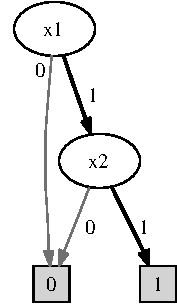
\includegraphics[%
    clip,
  scale=0.75]{obdd/figures/And1.pdf}&
&
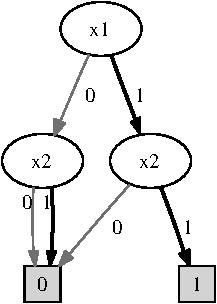
\includegraphics[%
  clip,
  scale=0.75]{obdd/figures/And1-full.pdf}\tabularnewline
Figure \ref{cap:BDDfill}(a)&
&
Figure \ref{cap:BDDfill}(b)\tabularnewline
\end{tabular}\end{center}
\caption{\label{cap:BDDfill}Adding dummy vertices}
\end{figure*}

One of the difficulties in developing and proving the protocol is
that OBDDs allow skipping of levels.  For example,
Figure~\ref{cap:BDDfill}(a) shows the OBDD for the Boolean function
$x_1 \wedge x_2$. Assume that the vertex at level $0$ is labeled with
$x_1$ and vertices at level $1$ are labeled with $x_2$. Suppose Alice
owns variable $x_1$ and Bob owns variable $x_2$. If Alice's input
is $1$, then Bob follows one more edge than if Alice's input were
$0$, which allows Bob to determine Alice's input. Compare this to
Figure~\ref{cap:BDDfill}(b), where a dummy vertex is added so
that, regardless of Alice's input, Bob has to follow the same number of
edges. In this case, Bob learns nothing about Alice's input. Before
Alice garbles the OBDDs, she adds dummy vertices so that each path
from the root to a terminal node has the same number of edges.  Alice adds
dummy nodes whenever $OBDD(f)$ allows Bob to skip levels when
evaluating the OBDD on his share of the input. Recall that the
$0$-successor and $1$-successor of $v$ is denoted by ${\it low}(v)$
and ${\it high}(v)$. For example, if node $n$ at level $j$ has node $n'''$ at level
$j+3$ as its $0$-successor, then Alice inserts two dummy nodes $n'$
and $n''$ at level $j+1$ and $j+2$ respectively. The $0$-successor of
node $n$ is changed to $n'$, both $0$ and $1$-successors of $n'$ are
set to $n''$, and both $0$ and $1$-successors of $n''$ are set to
$n'''$.

\vspace{2ex}
The steps of protocol 1 are as follows:

%\begin{center}
%\begin{boxfig*}{ht!}{
\textsc{\bf Input:} Both parties' inputs include the $OBDD(f)$ for the Boolean function
$f(x_1,x_2,\cdots,x_n)$ with the ordering $x_1 < x_2 < \cdots < x_n$.
Furthermore, Alice holds the inputs $(i_1,\ldots,i_k)$ corresponding
to the first $k$ variables $x_1,\ldots,x_k$, and Bob has the inputs
$(i_{k+1},\ldots,i_n)$. 
\vspace{1ex}
\begin{enumerate}
\item Alice performs the following steps:
\begin{enumerate}
\item She traverses the $OBDD(f)$ using her
input $(i_1,\cdots,i_k)$, which results in a node $v_{init}$ at level
$k$.

\item She uniformly and independently at random creates $(n-k)$ pairs
of secrets $(s_1^0,s_1^1),\cdots,(s_{n-k}^0,s_{n-k}^1)$.  In addition,
for each node $v$ in the $OBDD(f)$ whose level is between $k$ and $n-1$,
Alice also creates a secret $s_v$. 

\item She assigns a uniformly random label to each node whose level is
between $k$ and $n$. We refer to the randomly assigned label of node
$v$ using the notation $label(v)$.

\item Next, Alice augments $OBDD(f)$ with some number of dummy nodes
(to ensure that Bob always traverses $n-k$ nodes in his phase of the protocol). 


\item Alice garbles all nodes whose level is between $k$ and $n-1$
in the following manner. Let $v$ be a node in $OBDD(f)$ such $k \leq
{\it level}(v) \leq n-1$ and define ${\it level}(v)=\ell$. The encryption of node $v$, denoted
by $E^{(v)}$, is a label and a randomly ordered ciphertext pair
\[
\left(label(v)\,\,,\,\,E_{s_v \oplus s_{\ell-k+1}^0} (label(low(v)) \,\|\, s_{{\it low}(v)})\,\,\,,\,\,\,
E_{s_v \oplus s_{\ell-k+1}^1} (label(high(v)) \,\|\, s_{{\it high}(v)})\right)\,\,\,,
\]
where the labels are pre-pended to the secret with a separator symbol
and the order of the ciphertexts is determined by a fair coin
flip. Roughly speaking, the secrets corresponding to the $0$-successor
and $1$-successor of node $v$ are encrypted with the secret
corresponding to $v$ and its level.

Note that dummy nodes have the same structure as normal nodes, except
that the ciphertext pair contain encryptions of the same message since
dummy nodes have the same $0$ and $1$-successors. Provided the
encryption scheme is semantically secure, this poses no problem since
the keys are chosen uniformly at random.

Lastly, there are two terminal nodes of the form $(b,label(t_b))$ for
$b=0$ or $1$. Recall that $OBDD(f)$ has two terminal nodes, denoted as
$0$ and $1$, that are at level $n$.

\item Once Alice is done encrypting, she sends to Bob the encryption
of all nodes whose level is between $k$ and $n$ and the secret
$s_{v_{init}}$ corresponding to node $v_{init}$ at level $k$. We called
this the garbled OBDD.

\end{enumerate}

\item Bob performs the following steps:
\begin{enumerate}
\item He engages in $n-k$ 1-out-of-2 oblivious transfers to obtain the
secrets corresponding to his input. For example, if his input $i_j$ is
$0$, then he obtains the (level) secret $s_{j-k}^0$; otherwise, he
obtains the secret $s_{j-k}^1$.

\item Now Bob is ready to start his computation. Suppose
$i_{k+1}=0$. With $s_{1}^0$ and $s_{v_{init}}$, he decrypts both
ciphertexts in $E^{(v_{init})}$ and decides which gives the correct
result by using the verifiable range property of the encryption
scheme. Bob now has both $s_{{\it low}(v)}$ (the secret corresponding
to the $0$-successor of $v_{init}$) and $label(low(v))$ (which tells
Bob which encrypted node is used to evaluate his next
input). Continuing this way, Bob eventually obtains a label
corresponding to one of the terminal nodes, which determines the
result of the OBDD on the shared inputs. Bob sends this result to
Alice.
\end{enumerate}

\end{enumerate}
%}
%\vspace{-0.1cm}
%\caption{\label{protbasicobdd} Protocol 1.}
%\end{boxfig*}
%\end{center}

We prove correctness and security in the semi-honest threat model,
defined in section 2.1.  Claim~\ref{claim:protocol1correct}
proves that protocol 1 is
correct; that is, Bob computes the function $f(i_1,\cdots,i_n)$.
Claim~\ref{claim:protocol1secure} proves that protocol 1 is secure
in the semi-honest model; that is, at the end of protocol 1, Alice only
knows its input and the value of the function $f(i_1,\cdots,i_n)$, and
similarly for Bob. For our proofs, we require the definition of elusive range and
efficiently verifiable range from Lindell and Pinkas~\cite{LP04}.
\begin{definition}
Let \alg{(G},\alg{E},\alg{D)} be a symmetric key encryption scheme
with key-generation, encryption, and decryption algorithms.
Denote the range of the scheme by
$\alg{Range}_n(k)=\{E_k(x)\}_{x\in\binset^n}$. We say that
\begin{enumerate}
	\item \alg{(G},\alg{E},\alg{D)} has an \textbf{elusive range}
	if for every probabilistic poly-time machine A, every
	polynomial $p(\cdot)$, and all sufficiently large $n$,
	$\Pr_{k\from\alg{G(1^n)}}[A(1^n)\in\alg{Range}_n(k)]<1/p(n)$.

	\item \alg{(G},\alg{E},\alg{D)} has an \textbf{efficiently
	verifiable range} if there exists a prob. poly-time
	machine $M$ such that $M(1^n,k,c)=1$ if and only if
	$c\in\alg{Range}_n(k)$.
\end{enumerate}
\end{definition}

\begin{claim} If the encryption scheme has an elusive range and the
oblivious transfer protocol is secure, then Protocol 1 is correct for
semi-honest Alice and Bob.
\label{claim:protocol1correct}
\end{claim}
\begin{proof}
First we show that every node in the garbled OBDD sent to Bob can be
evaluated correctly. For an encrypted node $v$, let $c_0$ and $c_1$ be
the first and second ciphertext term. Suppose $k$ is the key that Bob
obtains to decrypt the ciphertext in node $v$. Because the
encryption scheme is elusive and all the keys used in the garbled OBDD
are chosen uniformly and independently at random, it follows
immediately that, except with negligible probability, only one
ciphertext in an encrypted node decrypts correctly; that is,
either $c_0\in\alg{Range(k)}$ or $c_1\in\alg{Range(k)}$ but not
both. Hence, except with negligible probability, every node in the
garbled OBDD can be evaluated correctly.

By induction, we show that the correct key is obtained for every node
input and output. The base case is the key $s_{v_{init}}$ and the 
keys $s^{i_{k+1}}_{k+1},\ldots,s^{i_{n}}_{n}$ (corresponding to Bob's
input) obtained from Alice through the $n-k$ oblivious transfers. The
inductive step at node $v$ assumes that the correct label (pointing
Bob to node $v$) and node key $s_v$ was obtained in the previous
step. Furthermore, the correct level key $s_l^{i_l}$ was obtained by
executing an oblivious transfer protocol. Since every node in the
garbled OBDD can be evaluated correctly and the garbled OBDD is built by
a semi-honest Alice, Bob obtains the correct label and key output at
node $v$, which concludes the inductive step. We can conclude that the
entire garbled OBDD can be evaluated to give the correct result.\footnote{
Note that the negligible probability of error during
decryption can be removed by Alice first checking that every encrypted
node decrypts correctly before sending the garbled OBDD to Bob.
}
\end{proof}



\begin{claim} If the encryption scheme is semantically secure and has an
efficiently verifiable elusive range, and the oblivious transfer
protocol is secure, then Protocol 1 is secure against semi-honest
Alice and Bob.
\label{claim:protocol1secure}
\end{claim}
\begin{proof} 

%[{\it Proof of Claim~\ref{claim:protocol1secure}}]

Intuitively, Bob's security follows directly from the security of the
1-out-of-2 oblivious transfer protocol he uses to obtain the secrets
corresponding to his input. Alice's security follows from both the
security of the oblivious transfer protocol (allowing Bob to only
obtain only one key per node) and the semantic security of the
encryption scheme (which allows Bob to only decrypt one entry in each
node). We now flesh out the details by providing a simulation proof
from Alice and Bob's view of the protocol. Let $x$ and $y$ be the
inputs of Alice and Bob respectively and $\Pi$ be a protocol for
secure-function evaluation of $f(x,y)$.  Let ${\sf VIEW}_A^\Pi (x,y)$
and ${\sf VIEW}_B^\Pi (x,y)$ be the view of Alice and Bob for the run
of the protocol $\Pi$ on input $x$ and $y$ (view of a party consists
of its input, output, and all messages it receives during the
execution of the protocol). In a simulation proof one needs to show
two probabilistic polynomial-time algorithms $S_A$ and $S_B$ such that
$S_A (x,f(x,y))$ and $S_B (y,f(x,y))$ are computationally
indistinguishable from ${\sf VIEW}_A^\Pi (x,y)$ and ${\sf VIEW}_B^\Pi
(x,y)$, respectively.  For a precise definition of a simulation proof
the reader should refer to~\cite[Chapter 7]{Goldreich:vol2}.

We first consider the case where Alice is corrupt. Alice's view in an
execution of Protocol 1 consists of her view of the oblivious transfer
protocol executions and the output of the function from Bob at the
end. We now build a simulator that simulates Alice's view given access
only to her input and output. Because the oblivious transfer protocol
is secure, there exists a simulator that can simulate the transcript
of Alice's view of the oblivious transfer protocol without knowing
Bob's input. On input $(i_1,\ldots,i_k, f(i_1,\ldots,i_n))$, the
simulator first simulates Alice's view of all $n-k$ executions of the
oblivious transfer protocol by repeatedly running the oblivious
transfer protocol simulator. Using a standard hybrid argument on the
transcripts of all $n-k$ executions oblivious transfer protocols, we
see that if the oblivious transfer protocol is secure, then the
distributions of the simulated and real combined transcripts of all
$n-k$ oblivious transfer executions are indistinguishable with
non-negligible probability.

Finally, the simulator writes $f(i_1,\ldots,i_n)$ on the transcript
of Alice's view. We now show that the distribution of the output $f$
is indistinguishable (except with negligible probability) from the
real output, which amounts to showing that Bob outputs
$f(i_1,\ldots,i_n))$ correctly on a real interaction. By the security
of the oblivious transfer protocol, Bob is provided with the correct
keys corresponding to its input during each execution of the oblivious
transfer protocol. Applying claim~\ref{claim:protocol1correct}, it
follows immediately that, except with negligible probability, Alice
obtains the correct output from Bob, except with negligible
probability. Therefore, the distribution of the simulated transcript
is indistinguishable, except with negligible probability, from a real
transcript, concluding the case when Alice is corrupt.

We now consider the case when Bob is corrupt. Given
$(i_{k+1},\ldots,i_n, f(i_1,\ldots,i_n))$, the simulator $\simu$ must
simulate both a garbled OBDD that Bob can use to correctly compute
$f(i_1,\ldots,i_n)$, and Bob's view of the $n-k$ executions of the
oblivious transfer protocol. We first show how $\simu$ simulates the
$n-k$ oblivious transfer protocol executions. As in the previous case,
because the oblivious transfer protocol is secure, there exists a
simulator that can simulate the transcript of Bob's view of the
oblivious transfer protocol without knowing Alice's input. Therefore,
$\simu$ simulates Bob's view of all $n-k$ executions of the
oblivious transfer protocol by running the oblivious transfer protocol
simulator $n-k$ times. Using a standard hybrid argument on the
transcripts of the oblivious transfer protocols, we see that if the
oblivious transfer protocol is secure, then the distributions of the
simulated and real transcripts of all $n-k$ oblivious transfer
executions are indistinguishable except with negligible probability.

We now show how $\simu$ builds a garbled OBDD that Bob can use to
successfully compute $f(i_1,\ldots,i_n)$. Since $\simu$ does not know
$i_1,\ldots,i_k$, it cannot generate the garbled OBDD according to the
protocol instructions. Instead, $\simu$ generates a garbled OBDD that
always evaluates to $f(i_1,\ldots,i_n)$ regardless of the keys
used. Such a garbled OBDD is built by first generating a chain of $n-k$
garbled nodes $n_{k+1},\ldots,n_{n}$ such that Bob's computation
starts at  $n_{k+1}$ and proceeds along the chain through
$n_{k+2}$ and so on, before ending at node $n_{n}$; note that there is
one such node for every level from $k+1$ to $n$. To ensure the
computation always proceeds along this chain, \textit{both}
ciphertexts in garbled nodes $n_{k+1},\ldots,n_{n-1}$ are encryptions
(under different keys) of the same label-key message such that the
label points to the next node along the chain and the node key
combined with the level key allows successful decryption of that node;
for example, simulated node $n_j$ for $k+1 \leq j\leq n-1$ has the
form
\[
\begin{array}{l}
\left( label(n_j)\,\,,\,\,E_{s_{n_j} \oplus s_{l}^0} (label(n_{j+1}) \,\|\, s_{n_{j+1}}) \right. \\
\left. E_{s_{n_j} \oplus s_{l}^1} (label(n_{j+1}) \,\|\, s_{n_{j+1}})\right)\,\,\,.
\end{array}
\]
Node $n_{n}$ is the terminal node and it is set to
$f(i_1,\ldots,i_n)$. Once $n_{k+1},\ldots,n_{n}$ is generated, the
simulator generates a number of ``fake'' nodes so that the simulated
garbled OBDD contains the correct number of nodes; this number can be
determined from $OBDD(f)$. Fake nodes are nodes whose ciphertext pair
contain encryptions under different keys of the same label-key
message; in a fake node, the label, the keys used to encrypt the
ciphertext pair, and the label-key message encrypted in the ciphertext
pair are chosen randomly.

All that remains is to show that the distribution of the simulated
garbled OBDD is indistinguishable from that of a real garbled OBDD. We
do this by using a standard hybrid argument over the nodes in the
garbled OBDD. Specifically, we run hybrid experiments with garbled OBDDs
where real nodes are replaced by simulated nodes. We define the hybrid
distributions such that $H_0(i_1,\ldots,i_n)$ contains the real
garbled OBDD and $H_{B}(i_1,\ldots,i_n)$ contains the simulated garbled
OBDD where $B$ is the number of non-dummy nodes in the real garbled
OBDD. We do not need to consider dummy nodes in our hybrid experiment
OBDDs because dummy nodes have the same distribution as the simulated
fake nodes and do not affect our argument.

We now define the hybrid garbled OBDD in experiment
$H_i(i_1,\ldots,i_n)$; the difficulty here is that the hybrid OBDD
contains both real and simulated nodes but must still allow Bob to
correctly compute $f(i_1,\ldots,i_n)$. First, we traverse the real
garbled OBDD and label a node as active if it is used by Bob in the
process of evaluating the OBDD and inactive otherwise. Note that there
will be only $n-k$ active nodes. Next, we order the nodes in the
garbled OBDD by their level with level $j+1$ nodes placed ahead of
level $j+2$ and so on; within the same level, nodes are ordered
arbitrarily. The hybrid OBDD is defined as follows: first take the real
garbled OBDD and replace the first $i$ non-dummy nodes as follows:
inactive nodes are replaced with simulated fake nodes. An active node
at level $j$ is altered by replacing its current ciphertext pair with
two encryptions of the label-key message corresponding to the next
active node at level $j+1$. These replacement ciphertexts are created
with the keys used to create the original ciphertext pair. Note that
the distribution of this altered active node is identical to that of
the simulated node $n_j$ in the node chain described above. It is easy
to see that a garbled OBDD built with this definition has the same
distribution as 1) a real garbled OBDD when $i=0$ (i.e. for $H_0$), and
2) a simulated garbled OBDD when $i=B$ (i.e. for $H_B$).

We are now ready to show that the distribution of the simulated
garbled OBDD is indistinguishable from that of a real garbled OBDD; that
is, we will show that
$\{H_0(i_1,\ldots,i_n)\}=\{H_{B}(i_1,\ldots,i_n)\}$. Suppose to the
contrary that the distributions are distinguishable; that is, there
exists a poly-time distinguisher $\disting$ that 
\[
\begin{array}{l}
\vert \Pr[\disting(H_0(i_1,\ldots,i_n))=1] - \\
\Pr[\disting(H_{B}(i_1,\ldots,i_n))=1]>1/p\vert
\end{array}
\]
 for some polynomial
$p$. Then there exists a $j$ such that 
\[
\begin{array}{l}
\vert
\Pr[\disting(H_{j-1}(i_1,\ldots,i_n))=1] - \\
\Pr[\disting(H_{j}(i_1,\ldots,i_n))=1]>1/pB\vert
\end{array}
\]

Using $\disting$, we now build an adversary that breaks the semantic
security of the encryption scheme used to encrypt the garbled
nodes. Recall in a semantic security game, the adversary sends two
messages $m_0,m_1$ to the challenger and receives the encryption of
$m_b$ for $b=\binset$; the adversary's goal is to determine $b$. Let
$n^j$ be the $j$th node and we denote its two ciphertext terms as
$c^{j}_0$ and $c^{j}_1$. Note that node $n^j$ in the hybrid OBDD in
distribution $H^*_{j-1}$ is a real garbled node, whereas the same node
for distribution $H^*_{j}$ is a simulated garbled node; specifically,
$c^{j}_0$ and $c^{j}_1$ in distribution $H^*_{j-1}$ are encryptions of
different label-key messages, whereas they are encryptions of the same
label-key message in distribution $H^*_{j}$. We exploit this fact to
build the adversary $\adver$ that breaks semantic security of the
encryption scheme.

First, $\adver$ creates the hybrid garbled OBDD corresponding to the
distribution $H^*_{j-1}(i_1,\ldots,i_n)$. One of the two ciphertexts
$c^{j}_0$ and $c^{j}_1$ in node $n^j$ is an encryption of the label
and key for the active node $n^{j+1}$, whereas the other ciphertext is
an encryption of the label and key for an inactive node. Let $\ell_0$
be the label-key message encrypted in $c^j_0$ and $\ell_1$ be that
encrypted in $c^j_1$. Next, $\adver$ sends $\ell_0$ and $\ell_1$ to
the semantic security challenger and receives $c^*$, which is an
encryption of either $\ell_0$ or $\ell_1$. Without loss of generality,
let $\ell_0$ be the label-key message (contained in ciphertext
$c^{j}_0$) that leads to the next active node. $\adver$ replaces
$c^j_1$ with $c^*$ in node $n^j$ in the garbled OBDD that it built in
the first step, and then feeds the altered OBDD together with the other
required inputs to the hybrid distinguisher $\disting$. Note that
$c^*$ cannot be decrypted with the node and level keys for node
$n^j$. This fact, however, does not prevent the garbled OBDD from being
evaluated correctly because $c^*$ replaces $c^j_1$, which contains the
label and key to an inactive node, and would not be successfully
decrypted while evaluating the garbled OBDD on the inputs
$(i_1,\ldots,i_n)$.

$\disting$ eventually outputs a result stating that the input is of
distribution $H^*_{j-1}$ or $H^*_{j}$. If $\disting$ outputs that the
input is of distribution $H^*_{j-1}$, then $\adver$ outputs that $c^*$
is an encryption of $\ell_1$; otherwise $\adver$ outputs that $c^*$ is
an encryption of $\ell_0$. Notice that if $c^*$ is an encryption of
$\ell_0$, then both ciphertexts in node $n^j$ are encryptions of the
same label-message, and the input to $\disting$ has distribution
$H^*_{j}$. Similarly, if $c^*$ is an encryption of $\ell_1$, then the
input to $\disting$ has distribution $H^*_{j-1}$. Since $\disting$
distinguishes between $H^*_{j-1}$ and $H^*_{j}$ with non-negligible
probability, we see that $\adver$ wins the semantic security game with
non-negligible advantage. Since we assume that the encryption scheme is
semantically secure, this implication is a contradiction, and there is
no such distinguisher $\disting$ that distinguishes between
$H_0(i_1,\ldots,i_n)$ and $H_{B}(i_1,\ldots,i_n)$; that is, the
distribution of the simulated garbled OBDD is indistinguishable from
that of a real garbled OBDD. Therefore, Bob's simulated view is
indistinguishable, except with negligible probability, to the real
view, concluding the proof.
\end{proof}



\subsection{Protocol 2}
\label{subsec:protocol2}

The protocol presented in this section allows both Alice and Bob to
possess arbitrary input sets instead of assuming that Alice (and also
Bob) holds either the first $k$ or the last $n-k$ input variables.  In
this new protocol, before garbling the OBDD, Alice can reduce the size
of the OBDD by eliminating vertices whose labels correspond to Alice's
inputs.  Let $f(x_1,\cdots,x_n)$ be the function to be computed and
$X_A$ denotes the inputs of Alice. Alice first computes the OBDD  for the restriction $f
\mid_{X_A}$ of $f$ for the variables in its input
set $X_A$. Alice then encrypts the reduced OBDD and sends it to
Bob. During the restriction operation, all vertices whose labels
correspond to Bob's input should be included. If this is not the case,
then there is a risk that different restrictions could produce
different numbers of nodes, which would leak information to Bob about
Alice's inputs. For example, in Figure~\ref{cap:BDDpe}(a), where
Alice's value is $0$, there are only 2 nodes, but in
Figure~\ref{cap:BDDpe}(b), there are 3 nodes.
Figure~\ref{cap:BDDpe}(c) shows the result of retaining extra
vertices, in which case there are 4 nodes regardless of Alice's
inputs. The description of this protocol is presented next.
The proof of correctness of this protocol
is almost identical to the one presented in
Section~\ref{sec:obdd-basicprotocol}. Example~\ref{example:protocol2} shows
an execution of this protocol on a small function.

\begin{figure*}

\begin{center}\begin{tabular}{cp{0.5in}p{1in}p{0.3in}c}
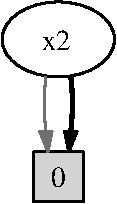
\includegraphics[%
  clip,
  scale=0.75]{obdd/figures/And1false.pdf}&
&
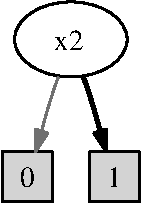
\includegraphics[%
  clip,
  scale=0.75]{obdd/figures/And1true.pdf}&
&
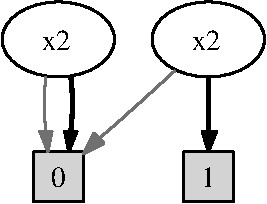
\includegraphics[%
  clip,
  scale=0.75]{obdd/figures/And1false2.pdf}\tabularnewline
Figure \ref{cap:BDDpe}(a)&
&
Figure \ref{cap:BDDpe}(b)&
&
Figure \ref{cap:BDDpe}(c)\tabularnewline
\end{tabular}\end{center}

\caption{\label{cap:BDDpe}OBDD restriction}

\end{figure*}

\vspace{2ex}
The steps of protocol 2 are as follows:

%\begin{center}
%\begin{boxfig}{ht!}{
\textsc{\bf Input:} Both parties' inputs include the $OBDD(f)$ for the Boolean function
$f(x_1,x_2,\cdots,x_n)$ with the ordering $x_1 < x_2 < \cdots < x_n$.
Furthermore, Alice holds the inputs for the variables in the set $X_A$ and
Bob holds the inputs for the variables in the set $X_B \; = \; \{ x_1,\cdots,x_n \} - X_A$.
\vspace{1ex}
\begin{enumerate}
\item Alice performs the following steps:
\begin{enumerate}
\item Alice computes the OBDD ${\cal O}_A$ for the function $f \mid_{X_A}$. This is the restriction
operation described in Section~\ref{sec:OBDDs}.

\item Alice encrypts the OBDD for the function $f \mid_{X_A}$ and sends it to Bob. This
step is exactly the same as for Protocol 1.  Alice also sends
the secret corresponding to the root of the OBDD ${\cal O}_A$. 


\end{enumerate}

\item The computation for Bob is exactly the same as that for Protocol 1. 

\end{enumerate}
%}
%\vspace{-0.1cm}
%\caption{\label{fig:protocol2} Protocol 2.}
%\end{boxfig}
%\end{center}


\begin{example}
\label{example:protocol2}
\rm Assume that Alice and Bob want to compute $f(x_1,x_2)  \; = \; x_1 \wedge x_2$, where
Alice has input $x_1$ and Bob has input $x_2$, or in other words $X_A
\; = \; \{ x_1 \}$ and $X_B \; = \; \{ x_2 \}$.  Assume that $x_1 = 0$
and $x_2 = 1$. $OBDD(f)$ with dummy nodes is shown in
figure~\ref{cap:BDDfill}(b). Alice computes the OBDD for the function
$f \mid_{ x_1 \leftarrow 0}$, which results in a structure shown in
Figure~\ref{cap:BDDpe}(c).  Let the two nonterminal nodes in
Figure~\ref{cap:BDDpe}(c) be $v_1$ and $v_2$. First, Alice generates
$2$ secrets $s_{v_1}$ and  $s_{v_2}$, which are assigned
to the nodes $v_1$ and $v_2$, respectively.   Alice also
generates random labels for the four nodes in
Figure~\ref{cap:BDDpe}(c), and  generates a pair of secrets
$(s_1^0,s_1^1)$. The garbled OBDD corresponding to
Figure~\ref{cap:BDDpe}(c) is shown below (terminal nodes
are shown as $0$ and $1$ and lab denotes label). 
\begin{center}
\begin{tabular}{|l|} \hline
$(lab(v_1), E_{s_{v_1} \oplus s_1^0} (lab(0)  \,\|\, s_0), E_{s_{v_1} \oplus s_1^1} (lab(0) \,\|\, s_0))$ \\ \hline
$(lab(v_2), E_{s_{v_2} \oplus s_1^0} (lab(0) \,\|\, s_0), E_{s_{v_2} \oplus s_1^1} (lab(1) \,\|\, s_1))$ \\ \hline
$(0,lab(0))$ \\ \hline
$(1,lab(1))$ \\ \hline
\end{tabular}
\end{center}
Alice reveals the secret $s_{v_1}$ corresponding node $v_1$.
Alice and Bob engage in a 1-out-of-2 ($OT^2_1$) protocol and Bob obtains the secret $s_1^1$ (recall that
$x_2 = 1$).
Bob can now decrypt the second component of the first entry of the garbled OBDD and
obtain $label(0) \,\|\, s_0$, and  Bob can infer that the output is $0$.
\end{example}

\begin{claim} If the encryption scheme has an elusive range and the
oblivious transfer protocol is secure, then Protocol 2 is correct for
semi-honest Alice and Bob.
\label{claim:protocol2correct}
\end{claim}
\begin{proof}
The proof of this claim is exactly same as the proof of Claim~\ref{claim:protocol1correct}.
One has to assume that the restriction operation used by Alice is correct.
\end{proof}

\begin{claim} If the encryption scheme is semantically secure and has an
efficiently verifiable elusive range, and the oblivious transfer
protocol is secure, then Protocol 2 is secure against semi-honest
Alice and Bob.
\label{claim:protocol2secure}
\end{claim}
\begin{proof}
%[{\it Proof Sketch for Claim~\ref{claim:protocol2secure}}]
The full proof is very similar for that in
Claim~\ref{claim:protocol1secure}, and we provide only a sketch. The
case when Alice is corrupt is identical to that in
Claim~\ref{claim:protocol1secure}. We briefly discuss why the proof is
also almost identical in the case when Bob is corrupt. The main
observation is that the simulator $\simu$ builds the simulated garbled
OBDD in the same way as in Claim~\ref{claim:protocol1secure} because
there is no difference in how Protocol 2 requires Bob to traverse the
garbled nodes given the same level keys. Therefore, the hybrid
distributions are defined the same way and the rest of the proof
follows.
\end{proof}


\section{Implementation and Experimental Results}
\label{sec:genomics-experimental}

In this section we present experimental results for our protocols for
computing the edit distance and the Smith-Waterman distance between
two strings.  For edit distance, our tests were performed on random
strings.  For the Smith-Waterman distance, we aligned representative protein
sequences from the Pfam database of protein sequences~\cite{pfam2002}
in protein family {\sf QH-AmDH\_gamma (PF08992)}, which is a
crystalline quinohemoprotein amine dehydrogenase from Pseudomonas
putida.  The average length of these proteins is 78 amino acids.  In
order to demonstrate the scalability of the algorithm, we truncate the
proteins to various lengths as shown in figure 6.  For a cost
function, we used the BLOSUM62 matrix~\cite{blosum62} which is a
$(20,20)$ substitution matrix based on log-odds statistics derived
from experimental protein data which approximates the probability of
substitution of amino acids in homologous proteins.  It is a commonly
used metric in genomic research.

\subsection{Edit distance}

% In this section, we describe our implementation of the three protocols
% for privately computing the edit distance between two strings and present
% experimental results for network bandwidth and execution times.

We implemented the standard methods for secure circuit evaluation,
\ie, the Yao's ``garbled circuits'' method and secure computation with
shares (see section~\ref{crypto}).  We used the oblivious transfer
protocol due to Noar and Pinkas~\cite{Naor-Pinkas:2001}.  For the
minimum-of-three computation, we used the lowest price auction circuit of
Kurosawa and Ogata~\cite{KO02}.  Using these primitives, we implemented
the three protocols of section~\ref{sec:protocols}.  For comparison
purposes, we also implemented the edit distance protocol of Atallah
\textit{et al.}~\cite{atallah}, using the Lin-Tzeng construction for
the millionaires' protocol~\cite{lintzeng-acns05} and Paillier homomorphic
encryption~\cite{Paillier99} (see appendix~\ref{appendix-atallah}).
All of the code was written in Java.

The experiments were executed on two 3-GHz Pentium 4 machines, with two
gigabytes of memory, and connected via a local LAN. Using this setup,
we obtained measurements (network bandwidth and execution times) for
the three protocols on various problem sizes. The reason for performing
the experiment on a local LAN is to provide a ``best-case'' result
for execution times in an environment where network bandwidth is not
a bottleneck.  Because the bandwidth numbers presented do not depend on
the experimental setup, execution times for bandwidth-limited networks
can be estimated from the numbers presented here.

The size of the problem instance is $(n,m)$, where $n$ and $m$
are the sizes of the two strings. For simplicity, all experiments
were performed on problems where $m=n$. The main conclusions that
can be drawn from our measurements are:

\begin{itemize}

\item \textit{Protocol 1 is not suitable for large problems.} 
Protocol 1 is ideal for small strings because the entire computation is
performed in one round, but the circuit size is extremely large for longer
strings.  We exhausted all available memory on our experimental machine
when evaluating a circuit for a problem instance of size $(26,26)$.

\item \textit{Protocol 2 can execute for problems of any size.} 
Protocol 2 performs reasonably well for moderate-size instances.
For example, a problem of size $(100,100)$ takes just under $9$ minutes
in our experimental setup.  Protocol 1 cannot scale to problems of
this size (although it is more efficient for very small problems).


\item \textit{Protocol 3 is most suitable for large problems.} 
Protocol 3 uses the grid structure of the problem space, which makes it
most suitable for large instances.  For example, a problem instance of
size $(200,200)$ takes under 10 minutes.  Asymptotically, protocol 3 has
the same performance as protocol 2, but in practice it is substantially
faster.  
\item \textit{Bandwidth requirements are asymmetrical.} 
Bandwidth requirements are asymmetrical.  Because Alice sends the
majority of data in the Naor-Pinkas~\cite{Naor-Pinkas:2001} oblivious
transfer protocol, bandwidth requirements are asymmetrical.
Specifically, Alice sends far more data than she receives and vice
versa for Bob.  This is useful because many real world communications
channels, such as ADSL or cable lines, offer a greater bandwidth for
transmitting data in one direction than in the other.  In this case,
the protocol would run with greater speed by assigning Alice's role to
the party that sends data faster, and Bob's role to the party that
receives data faster.


\item \textit{The edit distance protocol by Atallah et al.~\cite{atallah}
is not practical.} 
In our experiments, the protocol of~\cite{atallah} performed at least an
order of magnitude worse than our protocols.  This is because many large
numbers (Paillier ciphertexts) are computed and sent multiple times by
both Alice and Bob at each step.  For example, on problem instance of
size $(25,25)$ the protocol by Atallah \textit{et al.} took $5$ and half
minutes.  Our Protocol $3$ took $14$ seconds on the same problem instance.

\end{itemize}

Figure~\ref{fig:histogram} shows the execution times for our three
protocols. Clearly, protocol $3$ scales the best as the problem size
increases. Protocol $1$ is suitable for small problems. Protocol $2$
has a larger execution time, but only requires limited bandwidth per
round. Our experimental results confirm the protocol characteristics
shown in Figure~\ref{fig:protocol-characteristics}.

\begin{figure*}
\centerline{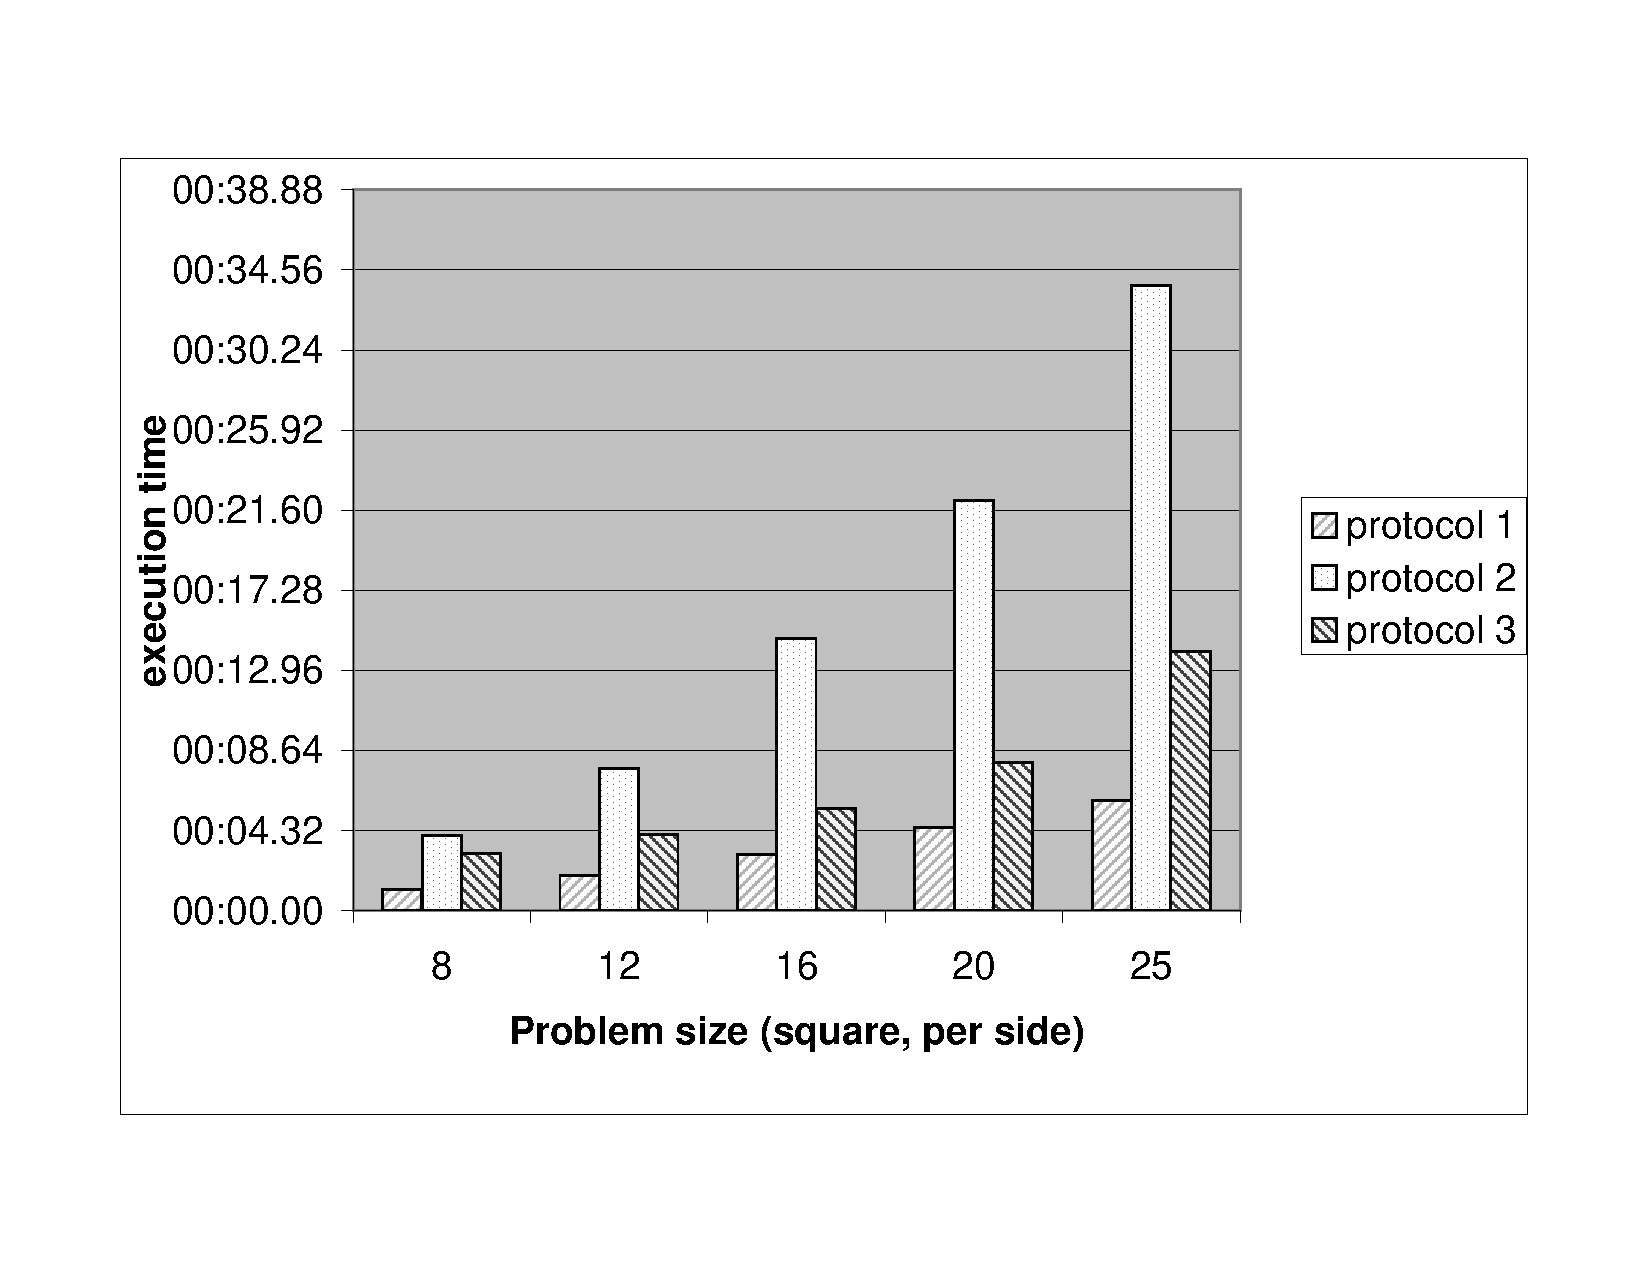
\includegraphics[bb=22bp -50bp 600bp 1000bp,scale=0.4,angle=0]{genomics/proto123}}
\caption{Timing measurements (in minutes and seconds) comparing protocols
1, 2, and 3. The Atallah~\cite{atallah} protocol could not complete problems of
sizes $(25,25)$ and $(25,25)$.}
\label{fig:histogram} 
\end{figure*}

Detailed results for protocol $1$ and $2$ are presented in the
appendix.  We discuss results for Protocol $3$ in detail. Recall that
in this protocol a grid structure is used (see
section~\ref{subsec:protocol3}).  Using Protocol $3$, we were able to
solve problems instances of considerable size; here we present
measurements for a problem instance of size
(200,200). Table~\ref{protocol3table200} shows the results using
various grid sizes. Performance steadily improves up to the grid size
of $20$, but begins to decrease slightly after that.  In spite of
decreased overall performance, further increases in the grid size
slightly decrease network bandwidth requirements, which results in
fewer round trips, so even larger grid sizes may be suitable for
environments with limited network bandwidth.  With a grid size of
$20$, Protocol 3 requires about as much time for an instance of size
$(200,200)$ as Protocol 2 requires for an instance of size ($25,25)$.


\subsection{Smith-Waterman}
\label{sec:sw-experimental}

For Protocols 1 and 3, the Yao circuit is modified by embedding the
cost function in the circuits. Recall that for edit distance, $\sigma=0$
if $\alpha[i]=\beta[j]$, $1$ otherwise. In Smith-Waterman, $\sigma$ is
an arbitrary cost function $c(u,v)$. The modified circuits effectively
perform a table lookup on $c(\alpha[i],\beta[j])$ in determining the
lowest cost alignment. Likewise, the gap function, which is a constant $1$
for edit distance, is replaced by the gap value of the scoring function
for Smith-Waterman. By convention, lower numbers represent higher costs
(higher numbers represent a similarity score) so a maximum-of-three circuit is
used instead of min-of-3.

We also constructed a protocol for Smith-Waterman based on Protocol
2. Recall that in Protocol $2$ for edit distance, a circuit for
equality of the characters is evaluated. For Smith-Waterman, an
$OT_{\mid \Sigma \mid}^{1}$ is performed instead. Alice, acting as the sender,
creates an array with a row of the cost function subtracted from her
random share $r$.  Each element of the array is $r-c(\alpha[i],\beta)$
for each possible $\beta\in\Sigma$. Bob, acting as the chooser, selects
the element with index $\beta[j]$. In this way, Bob receives the value
$r-c(\alpha[i],\beta[j])$.  Alice and Bob's shares are then input into
a maximum-of-three circuit which computes the next value of the shared dynamic
programming matrix.  The remaining details of the protocol are the same
as for edit distance.


Figure~\ref{fig:sw-histogram} shows the timing measurements for the
three protocols.  For Protocols 1 and 3, the computation time scales
with the size of the score matrix, which is ${\mid \Sigma \mid}^{2}$. For
example, the bytes transferred over the network aligning protein
sequences using BLOSUM62 are approximately 40 times that of for simple
edit distance of the same size problem.  This is caused by the use of
extra gates in the Yao circuit which encode each value of the score
function.  For Protocol 2, the computation scales with the alphabet
size $\mid \Sigma \mid$. For a very large alphabet with hundreds of symbols,
Protocol $2$ would be the best choice because the cost of embedding
the entire matrix into a Yao circuit becomes prohibitive.

\begin{figure*}
\centerline{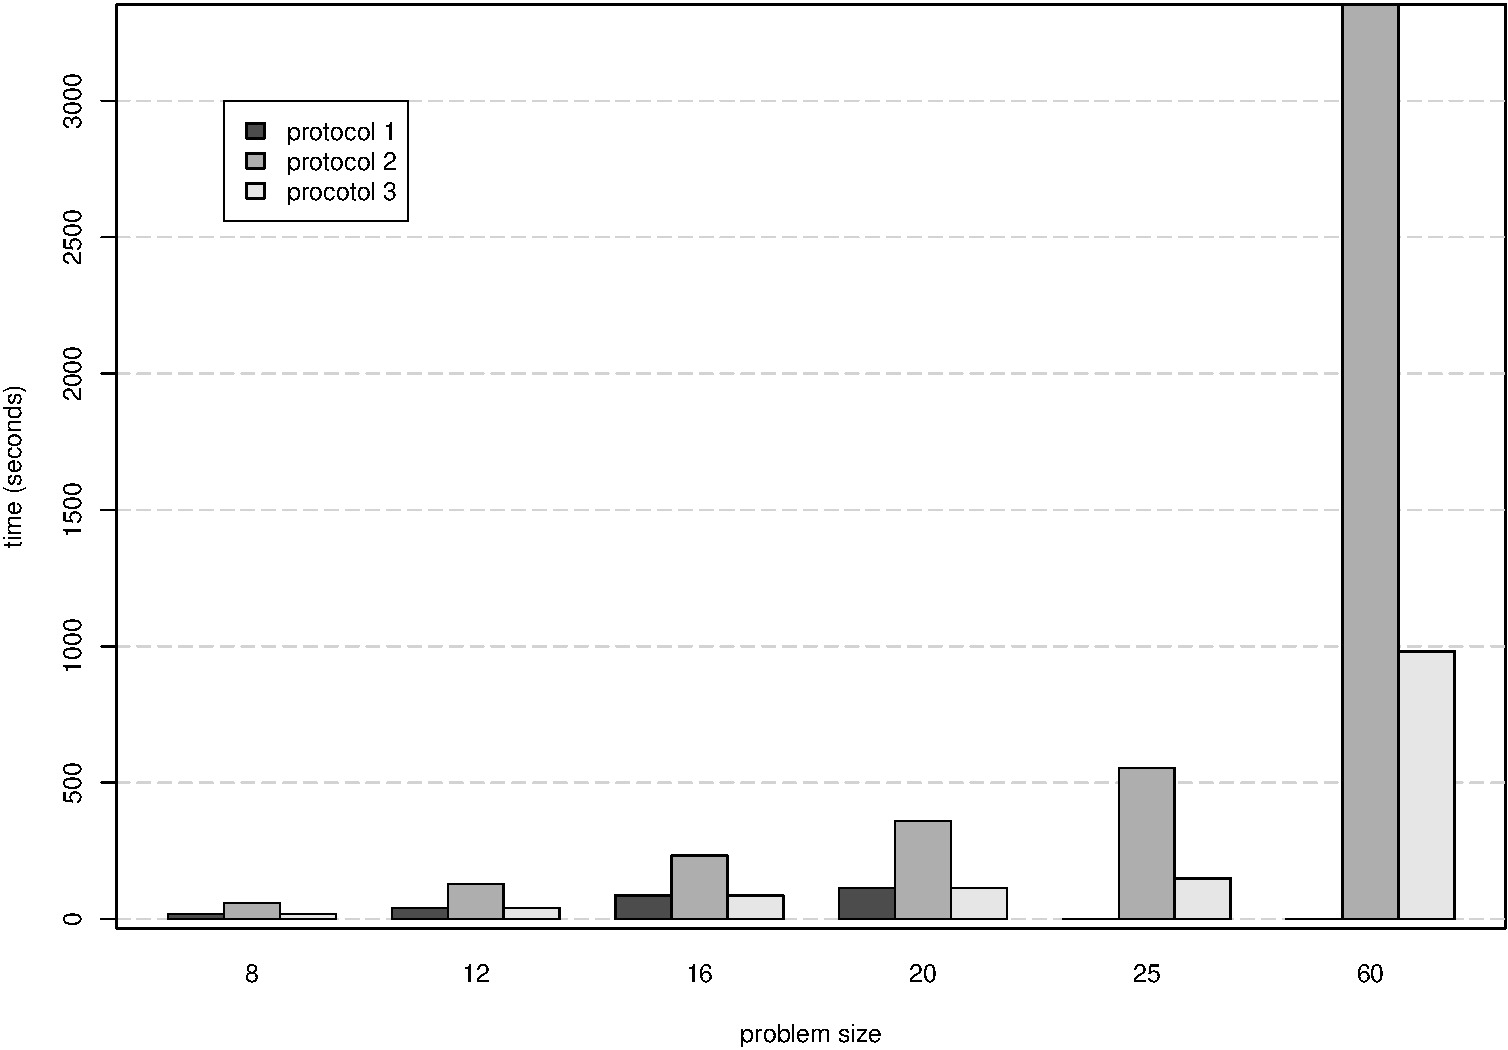
\includegraphics[scale=0.4,angle=0]{genomics/sw123}}

\caption{Timing measurements (in minutes and seconds) comparing Smith-Waterman
Protocols 1, 2, and 3. For problem sizes (25,25) and (60,60), Protocol
1 could not evaluate the circuit.}

\label{fig:sw-histogram} 
\end{figure*}

\begin{table}
\begin{centering}
\begin{tabular}{|c||c|c|c|c|c|}
\hline 
Grid size &
Bandwidth (Alice) &
Bandwidth (Bob) &
CPU (Alice) &
CPU (Bob) &
wall clock \tabularnewline
\hline
\hline 
25 &
362.2 M &
2.1 M &
518 &
84 &
658 \tabularnewline
\hline 
20 &
368.5 M &
2.6 M &
385 &
90 &
534 \tabularnewline
\hline 
10 &
397.4 M &
5.4 M &
476 &
123 &
655 \tabularnewline
\hline 
8 &
412.0 M &
5.8 M &
520 &
145 &
729 \tabularnewline
\hline 
4 &
485.3 M &
14.4 M &
784 &
234 &
1095 \tabularnewline
\hline 
2 &
635.2 M&
32.0 M&
1296 &
408 &
1804 \tabularnewline
\hline 
1&
948.0 M&
76.7 M&
2480 &
780 &
4883 \tabularnewline
\hline
\end{tabular}
\par\end{centering}

\caption{Network bandwidth (in bytes) and timing measurements (in seconds)
for edit-distance Protocol 3 with a problem of size $(200,200)$.
(M refers to Megabytes)}

\label{protocol3table200} 
\end{table}





%\section{Future Work}
\label{sec:future}


%% Say we should explore other representations and optimizations

There are other optimizations to OBDDs that we have not explored in
this paper. For example, adding negated edges to OBDDs can result in
smaller structures for some Boolean functions.\footnote{Following
a negated edge in an OBDD flips the value of the result.} Incorporating these
optimizations in our protocol while preserving privacy is a direction
for future work. There are several other OBDD-like representations
developed by the computer-aided design and computer aided
verification research communities, such as Binary Moment Diagrams
(BMDs)~\cite{BMD} and  Hybrid Decision Diagrams (HDDs)~\cite{HDD}. For a
certain class of functions, these representations are more succinct
than OBDDs. For example, BMDs can efficiently represent integer
multiplication, which cannot be represented efficiently at the
bit-level with OBDDs. Extending our protocol for these representations
is an important direction of future research. Our vision is to provide
an option for all these representations in our system so that a user can
choose the representation that is suitable for the problem.

%% Applications

OBDDs have been used for a variety of applications, such
efficient filtering in publish-subscribe systems~\cite{Jha:ICSE},
program analysis~\cite{Whaley}, and planning~\cite{Jensen}. In the future we
will investigate whether our protocol can be extended to design
privacy-preserving algorithms for these applications.


\begin{comment}
\bibliographystyle{plain} 
\bibliography{somesh,somesh-extra}

\appendix
\input{appendix-proofs}

\end{comment}
